% \subsection{Simulation data}

% The decode benchmark in this repository does not measure encoding. The fixture corpus is generated on the host first, and the benchmark binary measures only decoding. The data set contains:

% \begin{itemize}
%     \item 16 deterministic fixtures;
%     \item each fixture has one random 16-byte message;
%     \item each fixture has one corrupted HQC-128 codeword;
%     \item the Reed--Solomon symbol error count covers 0 through 15;
%     \item each codeword has 17664 bits, or 2208 bytes;
%     \item the expected output is the decoded 16-byte message.
% \end{itemize}

% If \texttt{HQC128\_BENCH\_ITERS=10}, then the total number of decodes is:

% \[
% 10 \times 16 = 160.
% \]

% \subsection{Simulation commands}

% Generate the fixture for the scalar version:

% \begin{lstlisting}[style=bashstyle]
% cd hqc_lab_scalar
% bash scripts/gen_hqc128_decode_fixture.sh
% \end{lstlisting}

% Run the decode benchmark on the host CPU:

% \begin{lstlisting}[style=bashstyle]
% bash scripts/run_hqc128_decode_bench_host.sh
% \end{lstlisting}

% Run the scalar version on the Hexagon simulator:

% \begin{lstlisting}[style=bashstyle]
% bash scripts/run_hqc128_decode_bench_hexagon.sh
% \end{lstlisting}

% Run the HVX intrinsic version on the Hexagon simulator:

% \begin{lstlisting}[style=bashstyle]
% cd ../hqc_lab_insintric
% bash scripts/gen_hqc128_decode_fixture.sh
% HQC128_BENCH_ITERS=10 bash scripts/run_hqc128_decode_bench_hexagon.sh
% \end{lstlisting}

% Run the HVX intrinsic version with the experimental GF LUT path:

% \begin{lstlisting}[style=bashstyle]
% HQC128_BENCH_ITERS=10 HQC_GF_LUT_MUL=1 \
%   bash scripts/run_hqc128_decode_bench_hexagon.sh
% \end{lstlisting}

% Note: the GF LUT path is faster in simulation, but it uses data-dependent table lookup. Therefore, it should not be the default cryptographic implementation if the threat model includes side-channel leakage.

\subsection{Simulation results}

The simulator benchmark uses the 16-fixture HQC-128 decode corpus and reports Hexagon Pcycles. The estimated cost per decode subtracts the fixed cost of the one-iteration run:

\[
\frac{\text{Pcycles}_{10\ \text{iters}} - \text{Pcycles}_{1\ \text{iter}}}{9 \times 16}.
\]

The following table reports the current working-tree full-decode simulator counters. The Pcycles/decode column is shown on the 10-iteration rows because it is derived from the paired 1- and 10-iteration measurements.

\begin{center}
\begin{tabular}{lrrrrr}
\toprule
Variant & Iters & Fixtures & Total instructions & Total Pcycles & Pcycles/decode \\
\midrule
Scalar & 1 & 16 & 15,658,009 & 17,830,458 & -- \\
Scalar & 10 & 16 & 139,902,579 & 155,172,882 & 953,767 \\
CT HVX intrinsic & 1 & 16 & 3,703,927 & 4,855,602 & -- \\
CT HVX intrinsic & 10 & 16 & 19,679,793 & 24,143,226 & 133,942 \\
Fastest non-CT HVX intrinsic & 1 & 16 & 3,193,630 & 4,285,368 & -- \\
Fastest non-CT HVX intrinsic & 10 & 16 & 8,048,619 & 11,271,900 & 48,518 \\
\bottomrule
\end{tabular}
\end{center}

Relative to scalar, the CT HVX intrinsic path is \(7.12\times\) faster in simulator Pcycles and reduces Pcycles/decode by 86.0\%.  The fastest non-CT HVX intrinsic path is \(19.66\times\) faster and reduces Pcycles/decode by 94.9\%, but remains a benchmark upper bound because it uses side-channel-relaxed control flow and data-dependent lookup tables.

\subsection{Substage analysis}

The substage benchmark was measured for all three simulator variants: scalar first, then default CT HVX, then fastest non-CT HVX.  RM substage costs are converted from per-block cost to per-decode cost by multiplying by 46 RM blocks.  RS substage costs are already per decode.

\begin{center}
\begin{tabular}{lrrr}
\toprule
Substage & Scalar & CT HVX & Fastest non-CT HVX \\
\midrule
RM expand/sum & 149,742 & 48,450 & 13,812 \\
RM Hadamard & 263,167 & 17,941 & 17,948 \\
RM find peak & 71,216 & 8,012 & 6,080 \\
RS syndrome & 162,309 & 8,358 & 8,358 \\
RS ELP & 119,591 & 44,879 & 6,574 \\
RS roots & 105,765 & 3,380 & 2,132 \\
RS Z polynomial & 13,044 & 11,145 & 1,141 \\
RS error values & 143,106 & 6,969 & 5,908 \\
RS correction & 439 & 439 & 427 \\
\midrule
Isolated substage sum & 1,028,378 & 149,572 & 62,380 \\
Full decode estimate & 953,767 & 133,942 & 48,518 \\
Substage sum / full decode & 107.8\% & 111.7\% & 128.6\% \\
\bottomrule
\end{tabular}
\end{center}

\begin{figure}[htbp]
\centering
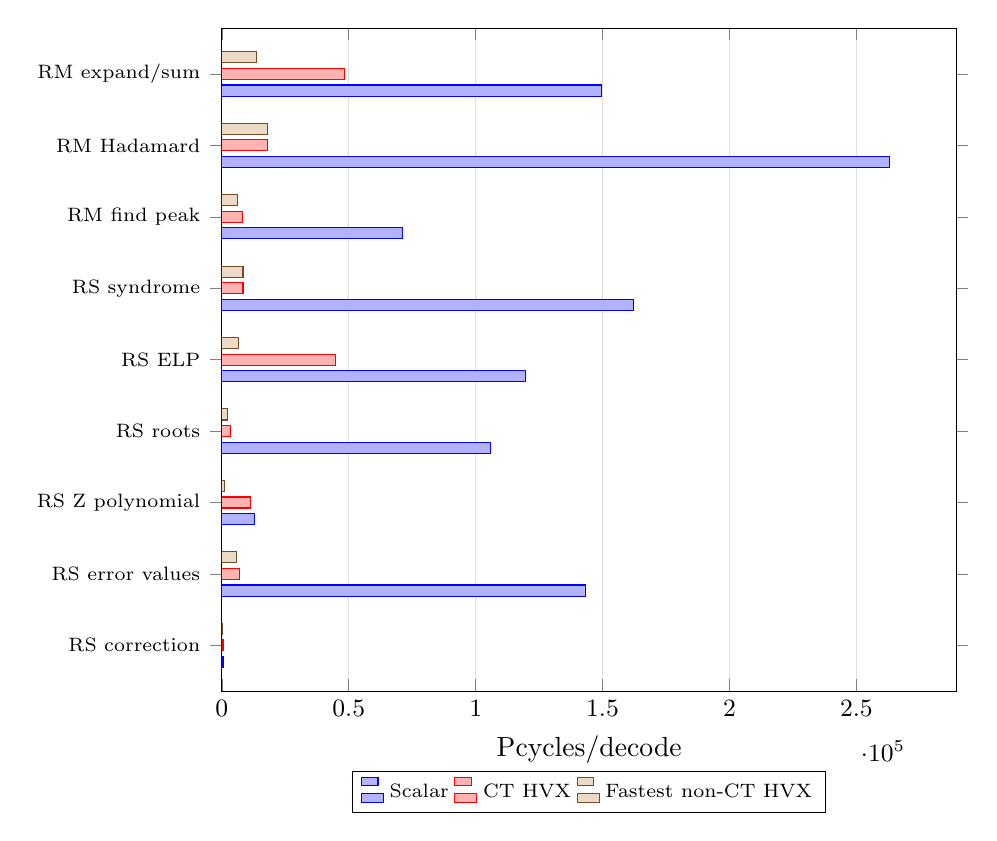
\begin{tikzpicture}
\begin{axis}[
    xbar,
    width=0.9\linewidth,
    height=10cm,
    bar width=4pt,
    xlabel={Pcycles/decode},
    symbolic y coords={RM expand/sum,RM Hadamard,RM find peak,RS syndrome,RS ELP,RS roots,RS Z polynomial,RS error values,RS correction},
    ytick=data,
    y dir=reverse,
    xmin=0,
    enlarge y limits=0.08,
    legend style={at={(0.5,-0.12)},anchor=north,legend columns=3,font=\scriptsize},
    x tick label style={font=\small},
    yticklabel style={font=\scriptsize},
    xmajorgrids=true,
    grid style={gray!25},
]
\addplot coordinates {
    (149742,RM expand/sum)
    (263167,RM Hadamard)
    (71216,RM find peak)
    (162309,RS syndrome)
    (119591,RS ELP)
    (105765,RS roots)
    (13044,RS Z polynomial)
    (143106,RS error values)
    (439,RS correction)
};
\addplot coordinates {
    (48450,RM expand/sum)
    (17941,RM Hadamard)
    (8012,RM find peak)
    (8358,RS syndrome)
    (44879,RS ELP)
    (3380,RS roots)
    (11145,RS Z polynomial)
    (6969,RS error values)
    (439,RS correction)
};
\addplot coordinates {
    (13812,RM expand/sum)
    (17948,RM Hadamard)
    (6080,RM find peak)
    (8358,RS syndrome)
    (6574,RS ELP)
    (2132,RS roots)
    (1141,RS Z polynomial)
    (5908,RS error values)
    (427,RS correction)
};
\legend{Scalar,CT HVX,Fastest non-CT HVX}
\end{axis}
\end{tikzpicture}
\caption{Grouped HQC-128 simulator substage costs. Lower is better.}
\end{figure}

The scalar breakdown shows that RM Hadamard, RS syndrome, RM expand/sum, and RS error values are the largest contributors before HVX optimization.  In the CT HVX path, the dominant remaining costs are RM expand/sum and RS ELP.  In the fastest non-CT path, RM Hadamard, RM expand/sum, and RS syndrome dominate the isolated breakdown.

\section{Real-device results}

The real-device measurements use the same 16-fixture decode corpus as the simulator benchmark, but report host-observed latency and direct device energy rather than simulator Pcycles. Each run performs 160,000 decodes. Energy is measured from Android power-supply voltage/current samples with qprof disabled; qprof is used only as diagnostic evidence for cDSP/NPU utilization and clock state.

\begin{center}
\begin{tabular}{llrrrrr}
\toprule
HQC & Backend & us/decode & uJ/decode & decodes/s/W & Speedup & Energy gain \\
\midrule
HQC-128 & CPU scalar & 80.622 & 217.929 & 4,674.205 & 1.00x & 1.0x \\
HQC-128 & NPU CT & 79.879 & 17.089 & 58,971.281 & 1.01x & 12.8x \\
HQC-128 & NPU fastest non-CT & 40.570 & 16.951 & 61,982.079 & 1.99x & 12.9x \\
HQC-192 & CPU scalar & 102.844 & 282.449 & 3,578.105 & 1.00x & 1.0x \\
HQC-192 & NPU CT & 90.681 & 36.433 & 27,447.467 & 1.13x & 7.8x \\
HQC-192 & NPU fastest non-CT & 50.734 & 21.245 & 48,012.445 & 2.03x & 13.3x \\
HQC-256 & CPU scalar & 227.041 & 655.251 & 1,531.320 & 1.00x & 1.0x \\
HQC-256 & NPU CT & 213.401 & 57.120 & 17,577.181 & 1.06x & 11.5x \\
HQC-256 & NPU fastest non-CT & 77.094 & 35.561 & 28,473.985 & 2.94x & 18.4x \\
\bottomrule
\end{tabular}
\end{center}

\begin{figure}[htbp]
\centering
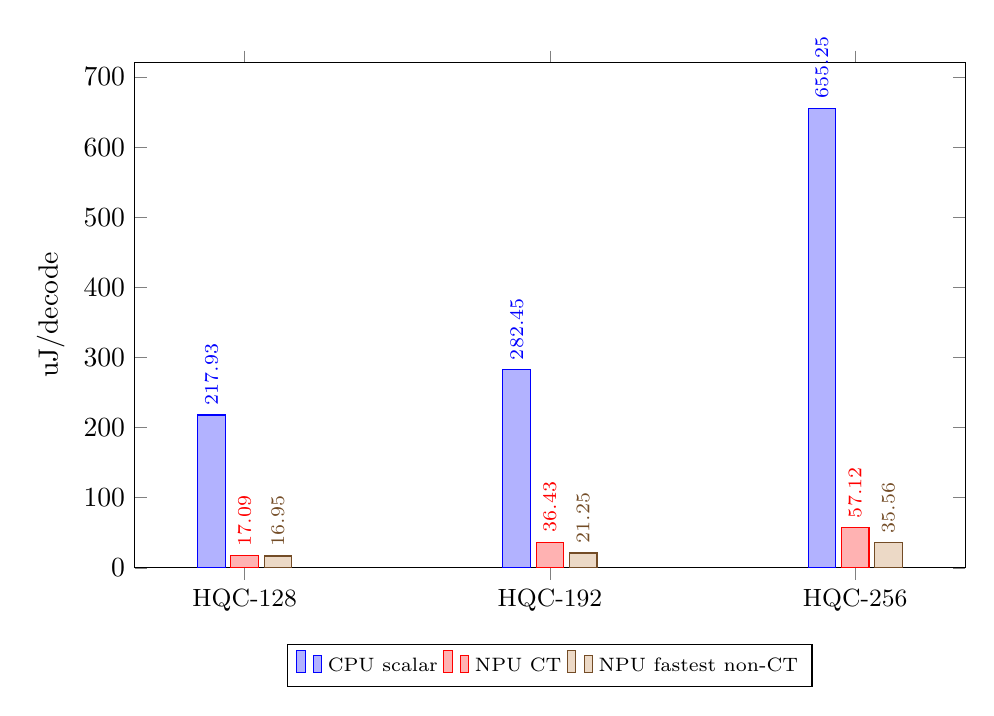
\begin{tikzpicture}
\begin{axis}[
    ybar,
    width=\linewidth,
    height=8cm,
    bar width=10pt,
    ylabel={uJ/decode},
    symbolic x coords={HQC-128,HQC-192,HQC-256},
    xtick=data,
    ymin=0,
    enlarge x limits=0.18,
    legend style={at={(0.5,-0.15)},anchor=north,legend columns=3,font=\scriptsize},
    nodes near coords,
    nodes near coords style={font=\scriptsize,rotate=90,anchor=west},
    yticklabel style={/pgf/number format/fixed},
    x tick label style={font=\small},
]
\addplot coordinates {
    (HQC-128,217.929)
    (HQC-192,282.449)
    (HQC-256,655.251)
};
\addplot coordinates {
    (HQC-128,17.089)
    (HQC-192,36.433)
    (HQC-256,57.120)
};
\addplot coordinates {
    (HQC-128,16.951)
    (HQC-192,21.245)
    (HQC-256,35.561)
};
\legend{CPU scalar,NPU CT,NPU fastest non-CT}
\end{axis}
\end{tikzpicture}
\caption{Real-device energy per decode. Lower is better.}
\end{figure}

The constant-time NPU implementation is the primary cryptographic result: it keeps latency close to, or slightly better than, the ARM64 CPU scalar baseline while reducing energy by 7.8x--12.8x. The fastest non-CT NPU path is a performance-oriented upper bound: it improves latency by 1.99x--2.94x and reduces energy by 12.9x--18.4x, but remains benchmark-only because it uses side-channel-relaxed control flow and data-dependent lookup tables.

\begin{center}
\begin{tabular}{llrrrr}
\toprule
HQC & Backend & process CPU \% & CPU ms/decode & CPU reduction & NPU util. \\
\midrule
HQC-128 & NPU CT & 0.096 & 0.0000625 & 99.922\% & 99.94\% \\
HQC-128 & NPU fastest non-CT & 0.452 & 0.0001875 & 99.766\% & 98.54\% \\
HQC-192 & NPU CT & 0.136 & 0.0001250 & 99.879\% & 99.59\% \\
HQC-192 & NPU fastest non-CT & 0.356 & 0.0001875 & 99.818\% & 98.87\% \\
HQC-256 & NPU CT & 0.110 & 0.0001875 & 99.917\% & 98.16\% \\
HQC-256 & NPU fastest non-CT & 0.161 & 0.0001250 & 99.945\% & 99.69\% \\
\bottomrule
\end{tabular}
\end{center}

The process-level CPU measurements show that the FastRPC/NPU paths reduce host CPU work by more than 99.7\% across all HQC levels, with process CPU utilization below 0.5\% in these runs. The qprof diagnostic runs report approximately 98.5\%--99.9\% NPU utilization with QDSP clocks around 1.16--1.18 GHz, confirming that the decode work is offloaded to the cDSP/NPU path. qprof power readings are excluded from energy claims because qprof can perturb clock and power state.
